\documentclass[12pt,a4paper]{article}

%-----------------------------------------------------------
% Packages & Configuration
%-----------------------------------------------------------
\usepackage[margin=1in]{geometry}
\usepackage{graphicx}
\usepackage{amsmath}
\usepackage{hyperref}
\usepackage{booktabs}
\usepackage{array}
\usepackage{xcolor}
\usepackage{titlesec}
\usepackage{fancyhdr}
\usepackage{enumitem}
\usepackage{float}
\usepackage{tabularx}
\usepackage{mdframed}
\usepackage{parskip}
\usepackage{microtype}
\usepackage{tikz}
\usetikzlibrary{shapes.geometric, arrows, positioning, shadows}

% Color Definitions
\definecolor{primaryblue}{RGB}{30, 64, 175}
\definecolor{accentgreen}{RGB}{5, 150, 105}
\definecolor{lightgray}{RGB}{248, 249, 250}
\definecolor{darkgray}{RGB}{31, 41, 55}

% Formatting Headers & Sections
\titleformat{\section}{\Large\bfseries\color{primaryblue}}{\thesection}{1em}{}[\titlerule]
\titleformat{\subsection}{\large\bfseries\color{accentgreen}}{\thesubsection}{1em}{}

% Page Headers/Footers
\pagestyle{fancy}
\fancyhf{}
\rhead{\textcolor{primaryblue}{\textit{Technical Flow Analysis}}}
\lhead{\textcolor{primaryblue}{\textbf{Wellbeing (WB-001)}}}
\rfoot{\thepage}
\lfoot{\textcolor{darkgray}{\footnotesize Healthcare Agentic OS | Flow Analysis v1.0}}

\hypersetup{
    colorlinks=true, linkcolor=primaryblue,
    urlcolor=accentgreen, citecolor=accentgreen,
    pdftitle={Wellbeing: Flow Analysis and Case Studies}
}

\begin{document}

\begin{titlepage}
    \centering\vspace*{1.5cm}
    {\Huge\bfseries\color{primaryblue} Flow Analysis \& Case Studies}\\[0.5cm]
    {\Large\color{accentgreen} Wellbeing: The Clinical Agentic OS}\\[1cm]
    {\large March 20, 2026}\\[2cm]

    \begin{mdframed}[backgroundcolor=lightgray, linecolor=primaryblue, linewidth=1.5pt, roundcorner=5pt]
        \centering\vspace{0.4cm}
        \textbf{Abstract:}\\[0.2cm]
        This document analyzes the operational flows of leading healthcare AI platforms (Abridge, Aidoc, Hippocratic AI, Microsoft Dragon Copilot, and Qure.ai) and contrasts them with the multi-agent, RAG-first architecture of \textbf{Wellbeing (WB-001)}. It provides a technical blueprint of the "Wellbeing Flow" and the integrated case studies.
        \vspace{0.4cm}
    \end{mdframed}
\end{titlepage}

\newpage
\tableofcontents
\newpage

\section{Introduction}
System flows are the critical pathways that determine how healthcare AI platforms ingest data, process clinical logic, and output verifiable results. This document synthesizes the flows from industry leaders to inform the development of \textbf{Wellbeing}, our Agentic OS.

\section{Case Studies: Competitor Flows}

\subsection{Abridge: Ambient Recording to Sign-off}
\begin{enumerate}[noitemsep]
    \item \textbf{Ambient Recording:} Clinical encounter captured in the background.
    \item \textbf{Contextual Reasoning:} Processes audio cross-referenced with EHR data.
    \item \textbf{Draft Note Generation:} Structured SOAP note appears in EHR.
    \item \textbf{Verification (Linked Evidence):} Every sentence is hyperlinked to audio for auditing.
    \item \textbf{Sign-off:} Clinician commits the note to the record.
\end{enumerate}

\subsection{Aidoc: Always-On Imaging Triage}
\begin{enumerate}[noitemsep]
    \item \textbf{Always-On Ingestion:} Monitors all incoming DICOM (CT/MRI) scans.
    \item \textbf{Autonomous Processing:} AI detects acute abnormalities (stroke, PE, ICH).
    \item \textbf{Prioritization:} High-urgency cases moved to the top of the radiologist's list.
    \item \textbf{Care Coordination:} Pushes real-time alerts to specialists' mobile apps.
\end{enumerate}

\subsection{Hippocratic AI: Proactive Patient Outreach}
\begin{enumerate}[noitemsep]
    \item \textbf{Need Identification:} Hospital identifies staffing gaps (e.g., chronic care management).
    \item \textbf{Automated Outreach:} AI voice agents initiate proactive outbound calls to patients.
    \item \textbf{Constellation Reasoning:} Multi-model architecture ensures non-diagnostic safety.
    \item \textbf{Clinical Escalation:} Supervisor agents trigger human handoff if risks are detected.
\end{enumerate}

\subsection{Microsoft Dragon Copilot: EHR-Native Documentation}
\begin{enumerate}[noitemsep]
    \item \textbf{EHR Launch:} Clinician starts the "Copilot" directly within Epic or Oracle.
    \item \textbf{Azure OpenAI Processing:} GPT-4 synthesizes the note from ambient audio.
    \item \textbf{Inline Correction:} Clinician edits the note within the native documentation field.
    \item \textbf{Integrated Billing:} System suggests CPT/ICD-10 codes based on documentation.
\end{enumerate}

\subsection{Qure.ai: Diagnostic Triage Flow}
\begin{enumerate}[noitemsep]
    \item \textbf{Image Acquisition:} Scan completed via hospital imaging hardware.
    \item \textbf{Triage Processing:} AI server analyzes DICOM file before human review.
    \item \textbf{Smart Notification:} Specialists alerted within seconds of critical findings.
    \item \textbf{Reporting Support:} Pre-filled reports with AI-detected highlights provided to doctors.
\end{enumerate}

\newpage

\section{Wellbeing: Our Bot Flow}
\textbf{Wellbeing (WB-001)} moves beyond static copilots to a state-managed, multi-agent orchestration.

\begin{figure}[H]
\centering
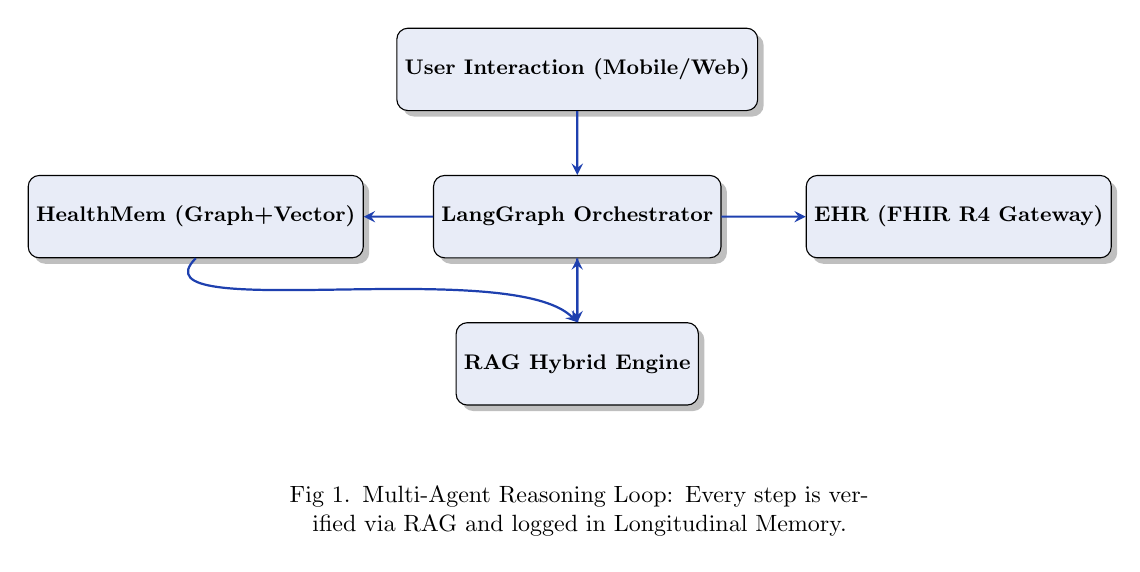
\begin{tikzpicture}[node distance=2.2cm, auto, scale=0.85, every node/.style={transform shape}]
    % Styles
    \tikzstyle{block} = [rectangle, draw, fill=primaryblue!10, text centered, rounded corners, minimum height=3.5em, minimum width=10em, font=\small\bfseries, drop shadow]
    \tikzstyle{arrow} = [thick,->,>=stealth, primaryblue]

    % Nodes
    \node [block] (ui) {User Interaction (Mobile/Web)};
    \node [block, below of=ui] (orch) {LangGraph Orchestrator};
    \node [block, below of=orch] (rag) {RAG Hybrid Engine};
    \node [block, right of=orch, xshift=3.5cm] (ehr) {EHR (FHIR R4 Gateway)};
    \node [block, left of=orch, xshift=-3.5cm] (mem) {HealthMem (Graph+Vector)};

    % Arrows
    \draw [arrow] (ui) -- (orch);
    \draw [arrow] (orch) -- (rag);
    \draw [arrow] (orch.west) -- (mem.east);
    \draw [arrow] (orch.east) -- (ehr.west);
    \draw [arrow] (rag) -- (orch);
    \draw [arrow] (mem.south) .. controls +(-1,-1) and +(-1,1) .. (rag.north);
    \node [below of=rag, text width=15cm, text centered] {Fig 1. Multi-Agent Reasoning Loop: Every step is verified via RAG and logged in Longitudinal Memory.};
\end{tikzpicture}
\end{figure}

\subsection{The Execution Flow}
\begin{enumerate}
    \item \textbf{Intent Classification (Orchestrator):} Parses user input into clinical triage, billing, or scheduling.
    \item \textbf{Context Retrieval (HealthMem):} Pulls longitudinal history (past 2 years of events) to avoid repetitive intake.
    \item \textbf{RAG-First Reasoning:} Fetches evidence from PubMed/Guidelines + Patient EHR Data.
    \item \textbf{Agent Collaboration:} Triage Agent hands off to Scheduling Agent to book the recommended follow-up immediately.
    \item \textbf{Source-Linked Generation:} Outputs the final result with clickable citations for clinician verification.
\end{enumerate}

\section{Comparison Summary}
\begin{table}[H]
\centering
\renewcommand{\arraystretch}{1.5}
\begin{tabularx}{\textwidth}{lXX}
\toprule
\textbf{Feature} & \textbf{Competitors (Avg)} & \textbf{Wellbeing (WB-001)} \\
\midrule
Flow Origin   & Hand-crafted Rules / Copilot & Agentic Multi-State Orchestration \\
Memory Layer  & Per-session or EHR-only & Longitudinal (Hybrid Graph+Vector) \\
Verification  & Probabilistic (LLM-based) & Deterministic Grounding (RAG-First) \\
Interop       & HL7 / FHIR APIs & Native Bidirectional FHIR Orchestration \\
\bottomrule
\end{tabularx}
\caption{Flow Differentiators}
\end{table}

\end{document}
